
\section{Electric Charges, Fields, and Potentials of a Point Charge}

\makelabheader %(Space for student name, etc., defined in master.tex)

\textbf{Objective}

\begin{itemize}
\item To investigate the electric field and potential of a point charge.
\end{itemize}

\textbf{Apparatus}

\begin{itemize}
%\item Electric field and potential simulation entitled {\it Charges and Fields}.
\item An internet browser with access to the Physics Education Technology (PhET) website
\end{itemize}

\textbf{Introduction}

The direction of an electric field is the direction of the force on
a tiny positive test charge placed in the region of space where the
field is to be measured. If the magnitude of this test charge is infinitesimally
small, so small that it will not displace or disturb the charges that
are the source of the field, we can use the test charge to determine
quantitatively the strength of the electric field. The strength of
the electric field is taken to be the electric force, $F$, on the test
charge divided by the magnitude of the test charge, \( q_{t} \):
\( E=\frac{F}{q_{t}} \). The magnitude of the force (Coulomb's Law) between two charges,
\( q_{1} \) and \( q_{2} \), is \( F=k\frac{q_{1}q_{2}}{r^{2}} \),
where \( k \)= 9 x 10\( ^{9} \) Nm\( ^{2} \)/C\( ^{2} \). The units
of \( E \) are newtons per coulomb, so another way of describing the field
strength is to say it is the force experienced by a unit positive
test charge.

Recall from a previous laboratory exercise that the potential difference
between two points A and B, V\( _{B} \) - V\( _{A} \), is the work
done carrying a unit positive charge from point A to point B. Also,
the lines of force (the electric field lines) are always perpendicular
to the equipotential lines, lines on which all points are at the same
potential. In a static electric field, the electric potential difference
between two points is a constant and does not depend on the path used
for its computation. The absolute potential, as opposed to the potential
difference, is the amount of work done in carrying a unit charge from
infinity to point B. The magnitude of the absolute potential, then,
is computed as the integral from infinity to the point B of the electric
field.

\textbf{Activity 1: The Electric Field of a Point Charge}

(a) To run the program {\it Charges and Fields} at the Physics Education Technology (PhET)
website go to the following address {\tt https://phet.colorado.edu/en/simulation/charges-and-fields}.
Click the {\it Download} button to start the program in your browser.
A blank `table top' with a set of menu 
buttons will appear. See Figure 1 below for an example.
If you don't see this consult your instructor.

\begin{figure}[hbt]
\begin{center}
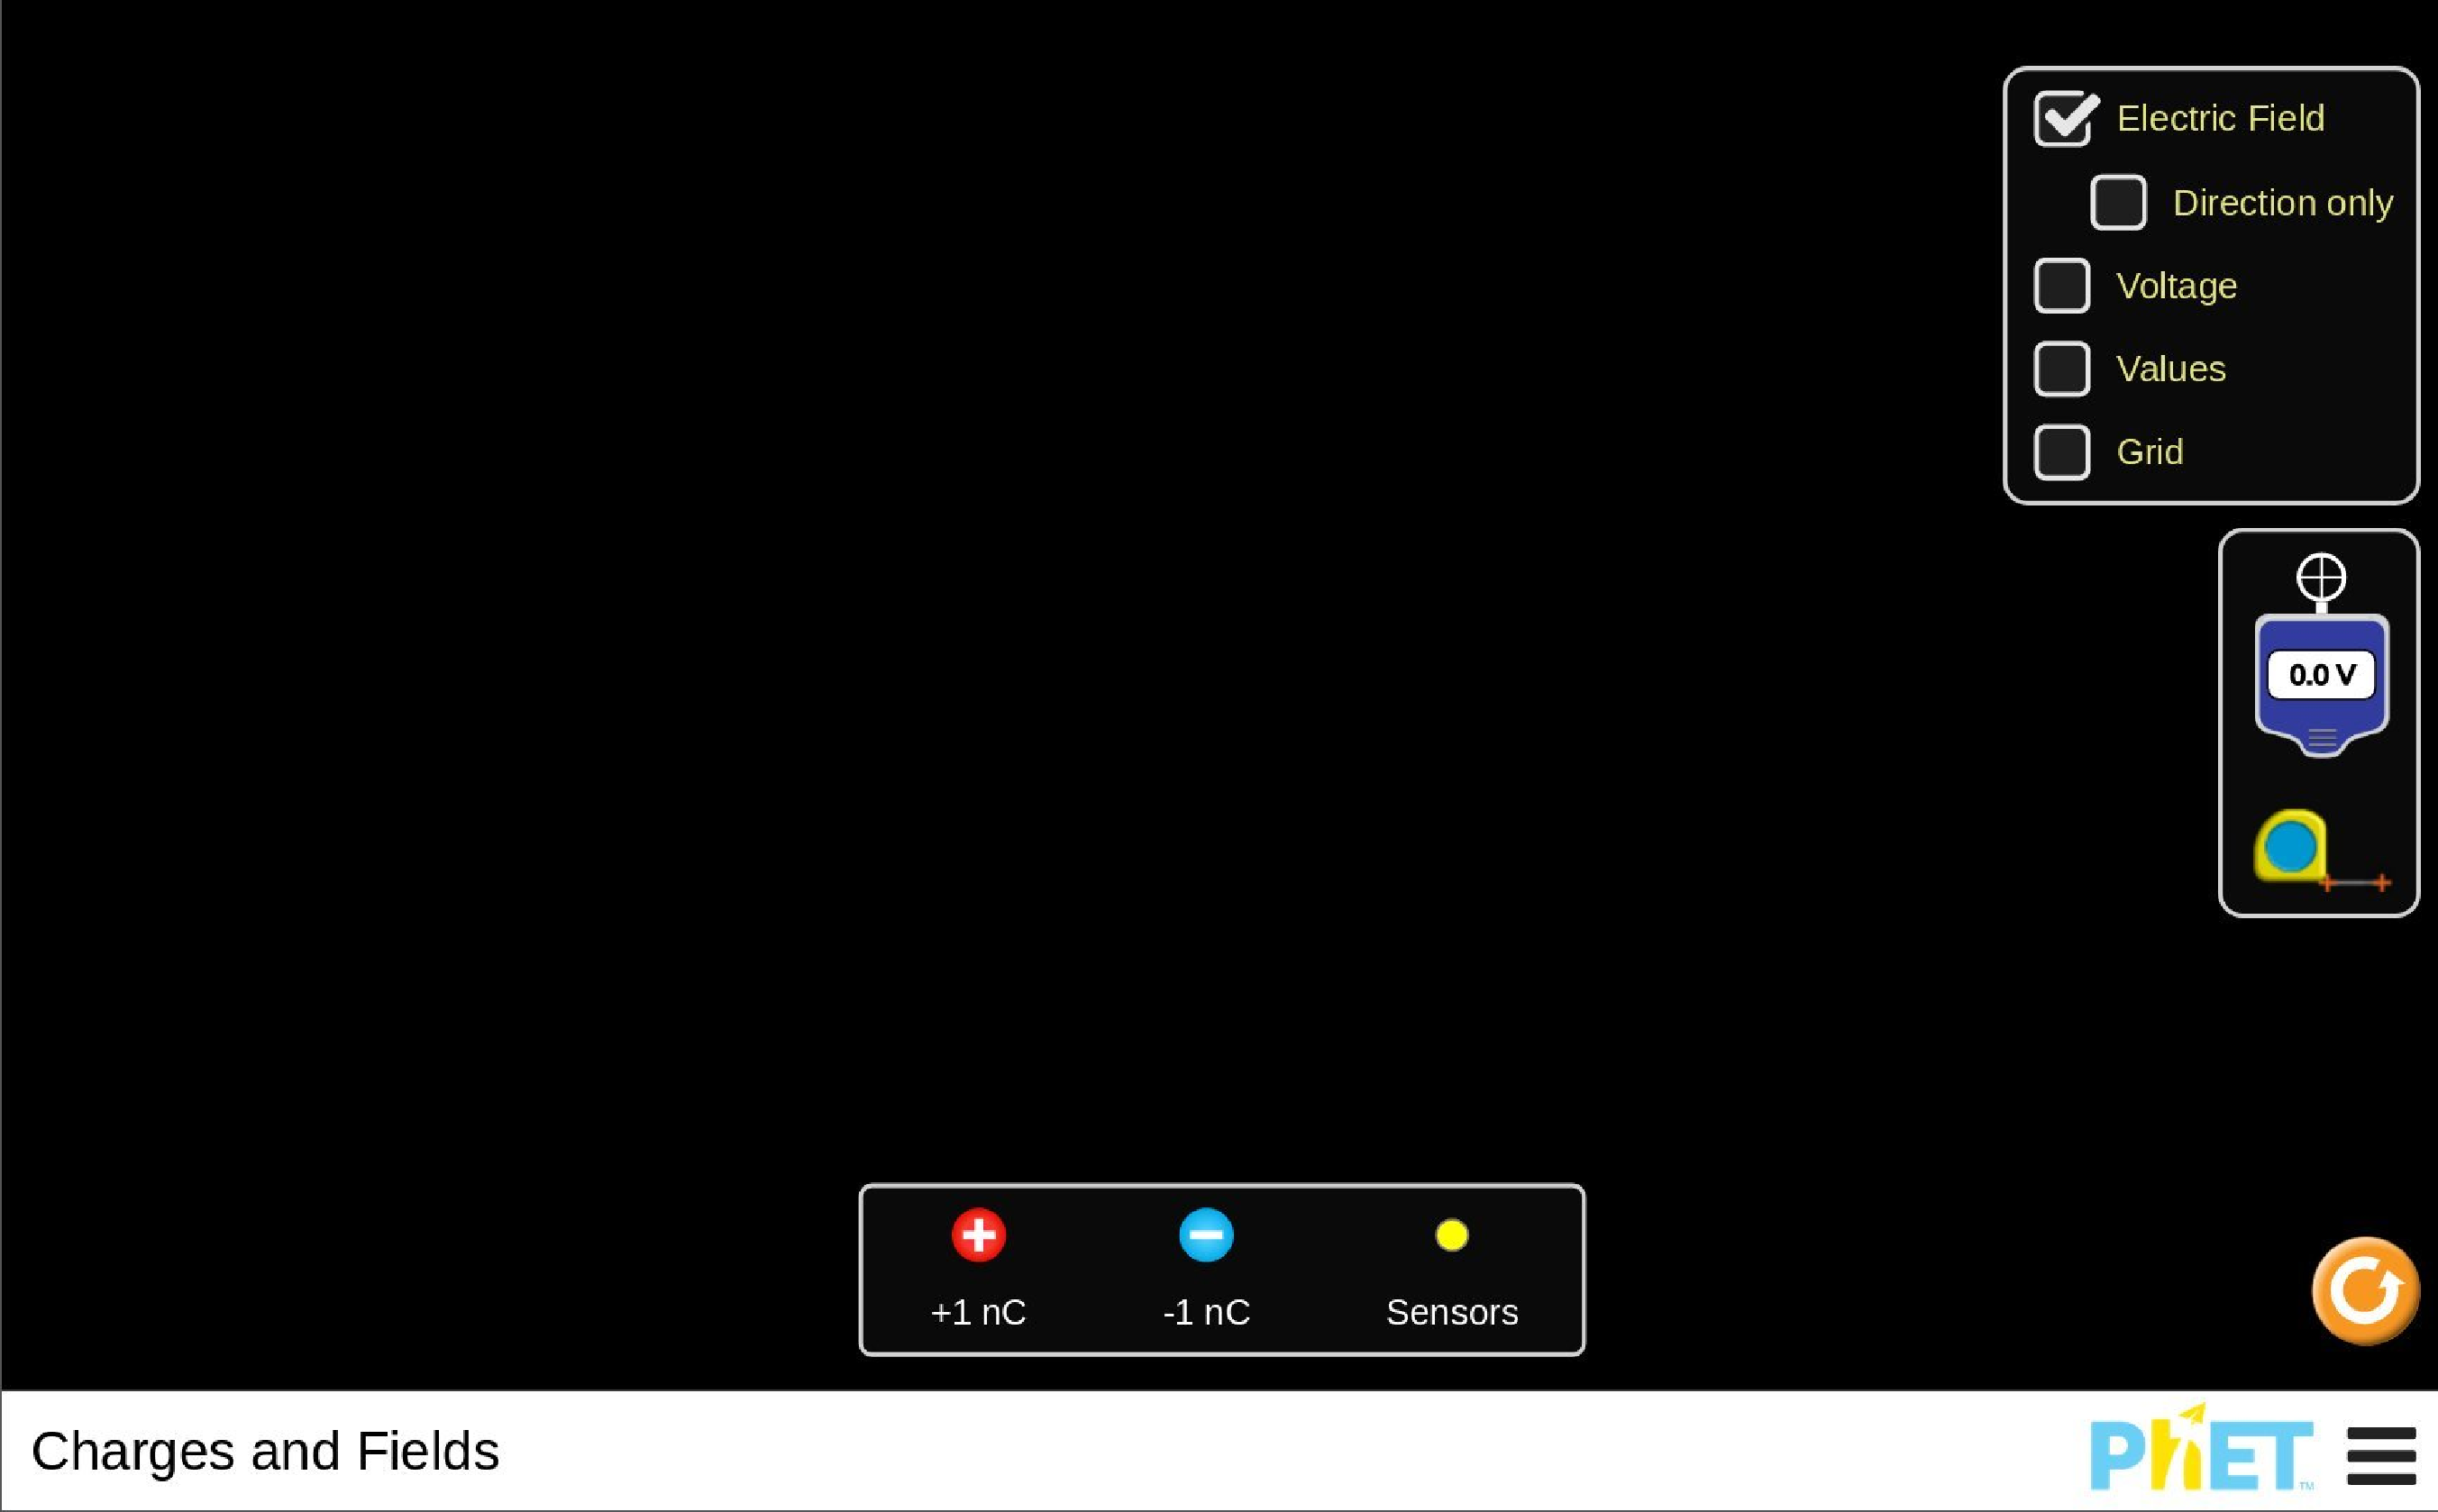
\includegraphics[height=3.0in]{chargesFields1/chargesFieldFig1.pdf}
\caption{Table top for {\it Charges and Fields.}}
\index{color page}
\end{center}
\end{figure}

(b) Go to the check boxes at upper-right on the table top and make sure only the {\tt Electric Field}
one is checked.

(c) Select the charge labeled {}``+1 nC'' from the available set by clicking
on it and dragging it onto the table top. 

(d) \textbf{Prediction}: You will take measurements of the field at different
distances from the charge. You know the size of the
charge (+1 nC).
Generate an expression for the magnitude of the field from this charge
with appropriate numerical constants and units.
How does the electric field depend on $r$, the distance from the point charge?
%\vspace{15mm}
\newpage

\vspace{-30mm}

(e) Click and drag one of the sensors (bottom-center of the table top)
to any point on the table top and release. You will see an arrow drawn.
The size and direction of the arrow represent the magnitude and direction of
the electric field at that point due to the `+1 nC' charge.
In what direction does the arrow point?
Click and drag another sensor to the opposite side of the table top.
In what direction does this arrow point? How is it related to the first arrow?
\vspace{15mm}

(f) Place many sensors on the table top so that you get a wide range of 
magnitudes from large
(barely fits on the table top) to small (barely visible outside the sensor).

(g) On the right-hand side of the table top click the {\tt Values} box. 
You should see values of the magnitude of the electric field appear near each
electric field vector.

(g) Drag the {\tt Tape Measure} on the right-hand side of the table top over to
your charge.
Click and drag one of the crosses on the {\tt Tape Measure} to the center of your charge.
Click and drag the other cross to the center of one of your sensors to get
the distance between the crosses.
Do this for all your sensors and enter these data in the table below. 
Print the table top and attach it to this unit.

\vspace{0.3cm}
{\centering \begin{tabular}{|c|c|c|c|}
\hline 
~~~Distance from Charge (cm)~~~&
~~~Measured E (N/C)~~~\\
\hline
\hline 
&
\\
\hline 
&
\\
\hline 
&
\\
\hline 
&
\\
\hline 
&
\\
\hline 
&
\\
\hline 
&
\\
\hline 
&
\\
\hline 
&
\\
\hline
\end{tabular}\par}
\vspace{0.3cm}

%(h) Use the results in column 3 of your table to determine the unknown charge 
%for each electric field measurement and enter the results in the table. NOTE: 
%For this calculation, assume the Coulomb's Law constant $k = 1.00 Nm^{2}/C^{2}$.
%This makes the charge a factor of about $10^{10}$ bigger than it is supposed to 
%be, but we are focussing here on how the electric field varies with distance 
%from the charge. Calculate the average and standard deviation of the values 
%of the charge. Are your results consistent? Explain.
%\vspace{30mm}

\newpage

(h) \textbf{Prediction}: From Coulomb's Law, we expect the spatial variation
of the field strength to obey a power law: \( \left| E\right| =Ar^{n} \),
where \( A \) and \( n \) are constants. What do you predict the value of 
\( n \) to be?\vspace{15mm}

(i) Graph the electric field strength you just measured as a function of $r$. 
Using the power fitting function, determine the power of the function, $n$, and record it here.
Attach the plot to this unit.
\vspace{12mm}

(j) Does your result agree with your prediction? Explain any discrepancy.
\vspace{12mm}

\vspace{0.5in}
\textbf{Activity 2: The Electric Potential}

(a) Click the yellow {\tt Reset} button in the lower-right corner of the table top
to erase the electric field vectors. Place another ``+1 nC'' charge on the table top.
Turn off the electric field vectors using the check box on the right-hand side.

(b) \textbf{Prediction}: You will now take measurements of the electric potential (or voltage).
How do you expect the electric potential to change with distance from the point
charge?
\vspace{15mm}
 
(c) Click and drag the cross-hairs on the {\tt Voltmeter} on the right-hand side of the table top.
Place the {\tt Voltmeter} on the table top and you can read the voltage
at the position of the cross-hairs.
Use the {\tt Tape Measure} to obtain the distance from the point charge to the cross-hairs.
Measure the electric potential and distance at many spots on the table top from very close to the point charge to
far away and record them in the table below.
When you are finished print the table top.
\vspace{5mm}

\vspace{0.3cm}
{\centering \begin{tabular}{|c|c|}
\hline 
~~~Distance (cm)~~~&
~~~Measured V (volts)~~~\\
\hline
\hline 
&
\\
\hline 
&
\\
\hline 
&
\\
\hline 
&
\\
\hline 
&
\\
\hline 
&
\\
\hline 
&
\\
\hline 
&
\\
\hline 
&
\\
\hline
\end{tabular}\par}
\vspace{0.3cm}


%(e) Calculate the value of the electric potential at each of these points
%from the distance you measured from the point charge and the value of the 
%charge from the previous activity. Again, assume $k = 1.00 Nm^{2}/C^{2}$.
%Fill in the appropriate columns of the table  with the distance
%and predicted potential. Show a sample calculation in the space below.
%\vspace{1in}


%(f) Did the measured values agree with your calculations? If they didn't,
%can you explain why not?\vspace{25mm}

(e) \textbf{Prediction}: From Coulomb's Law and the definition of the
electric potential, we expect the spatial variation of the potential
to obey a power law: \( \Delta V=Br^{m} \), where \( B \) and \( m \)
are constants. What do you predict the value of \( m \) to be?
\vspace{12mm}

\newpage

(f) Graph the voltage as a function of $r$. Using the power fitting
function, determine the power of the function, $m$, and record it here.
\vspace{12mm}

(g) Does your result agree with your prediction? Explain any discrepancy.
\vspace{12mm}

\textbf{Activity 3: Field Lines and Equipotentials}

(a) Clear the table top by clicking the yellow {\tt Reset} button at lower-right.
Place another ``+1 nC'' charge on the table top.

(b) Check the {\tt Electric Field} box on the right-hand side of the table top
and leave the other boxes empty.
Drag the charge around the table top.
What happens to the electric field arrows?
What direction do they point relative to the charge?
\vspace{30mm}

(c) Use the {\tt Voltmeter} on the right-hand side and place the cross-hairs
on the center of one of the field arrows. 
Click the {\tt Pencil} icon on the {\tt Voltmeter}.
The program draws a curve where all of the points are at the same electric potential.
This curve is the equipotential.

(d) Repeat these procedure at different distances from the point charge.
Why are they all circular?
\vspace{30mm}

(e) What is the relationship between the field lines and the equipotentials at 
the points where they cross?
